\documentclass[a4paper]{report}
\usepackage[english]{babel}
\usepackage{amssymb}
\usepackage{amsmath}
\usepackage{graphicx}
\usepackage{float}
\usepackage{shortvrb}
\usepackage{cancel}
\usepackage[T1]{fontenc}
\usepackage{nicefrac}
\usepackage{amsfonts}

%nomenclature
\usepackage{makeidx}
\makeindex
\usepackage{nomencl}
\nomlabelwidth=20mm
\makenomenclature
\renewcommand{\nomname}{List of abbreviations}

\usepackage{standalone} %Makes it possible to ignore other preambles of child document
\usepackage{eurosym} %Euro teken mogelijk
\usepackage{multirow} %For multiple rows togheter in one table
\usepackage{parskip} %For a small white line between paragraphs
\usepackage[protrusion=true,expansion=true]{microtype}
\usepackage{hyperref}%For automatic and URL Reference
\usepackage[titletoc]{appendix}
%Possible to change the margins
\usepackage{geometry}
\geometry{verbose,tmargin=1.9cm,bmargin=1.7cm,lmargin=1cm,rmargin=1cm}

\usepackage{subfig}

%include pdf pages
\usepackage{pdfpages}

%being able to create tables over multiple pages
\usepackage{longtable}

\makeatletter

%Change standard font size
\renewcommand\normalsize{ \@setfontsize\normalsize{11pt}{11pt}}\normalsize  
\makeatother

\usepackage{fancyhdr}
\pagestyle{fancy}
\fancyhead{}
\fancyfoot{}

%Gives text above each page
\fancyhead[CO,CE]{DSE Project}

%Page number
\fancyfoot[RO,LE]{\thepage}


\usepackage{babel}

%Available structures:
%Report: \part{}, \chapter{}, \section{}, \subsection{}, \subsubsection{}, \paragraph{}, \subparagraph{}

\begin{document}
\chapter{Risk management}
All risks that can occur during the design process are divided into four subgroups, namely cost risks, organizational risks, technical risks and schedule risks. Together they form the management risk. An overview of all the risks is shown in the Risk mind map which can be found in \autoref{fig:riskmindmap}\\

\begin{figure}[H]
\label{fig:riskmindmap}
\centering
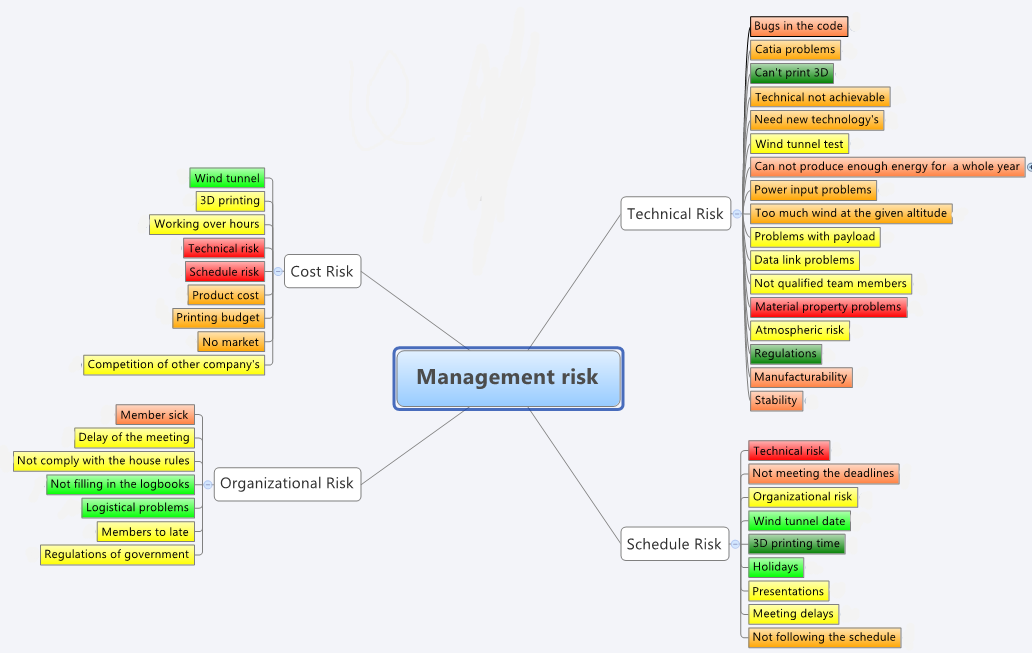
\includegraphics[scale=0.6]{Figures/Riskmindmapmain.png}
\caption{The main risk assessment }
\end{figure}

Each risk is given a specific colour related to its importance and influence on the design process, similar to the colours (and their meaning) used in the Risk Map. Thus the more red the colour of a risk the more important it is for the overall design process. Next to the risks a solution is suggested to solve for the occurring problem. Some of these solutions may seem pretty trivial, but that is because some things can be resolved quite easily. Only when something goes wrong, it will be clear whether the suggested solution indeed solved the problem or not. From this experience better solutions might be found and the risk mind map will be adapted. This way future incidents can be better prepared for. \\
Some sub group risks are noted as a risk in another sub group. For instance technical risk is mentioned as a risk in the schedule risk sub group. This is because they are linked to each other. If something goes wrong within the technical risk department, clearly it has an influence on the scheduling since extra work needs to be done in order to solve the technical problem. This linking of subgroups can be seen in the cost sub group as well. When things need to be rescheduled or technical problems arise, it will affect the costs as well.

\section{Risk map}
The technical risks that are identified with the project are plotted in a Risk Map. A Risk Map indicates the chance or likelihood of risks occurring and how severe they are. This is done by indicating on one axis the likelihood  and on the other axis the impact. The Risk Map can be found in \autoref{fig:riskmap}. \\
\begin{figure}[H]
\label{fig:riskmap}
\centering
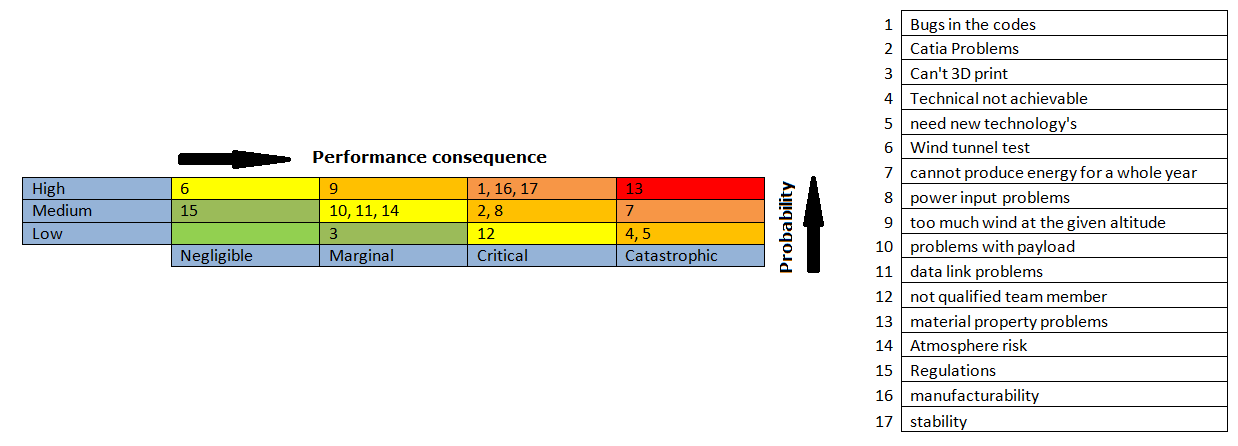
\includegraphics[width=\textwidth]{Figures/riskmap.png}
\caption{The technical risk map }
\end{figure}

Only three levels of probability have been chosen to indicate the likelihood; high, medium and low. This is done to make a clear distinction between the probabilities of each risk. Also at this stage of the design it is difficult to better predict the likelihood. Later on in the design process, the probabilities can be better predicted and the Risk Map will be adapted accordingly. \\
The levels of consequence are negligible, marginal, critical and catastrophic in increasing order of impact respectively. If some technical risk is assigned a negligible consequence, it doesn't mean it is in fact completely negligible. It just means it doesn't have as large an influence on the design process. Some risks that have a high probability of occurrence but negligible impact still need to be addressed. Of course risks that have catastrophic consequences are most important. \\
In the top right corner, indicated with a red region, the risks are shown that have a high probability of occurrence and a large impact on the design process. These are the most important ones and have the largest influence on the design process. On the other hand in the bottom left corner, indicated with a green region, risks are shown that have a small chance of occurrence and little consequence on the design process. These have a minimal influence on the design process. \\
With the aid of the Risk Map the technical risks are assessed on regular basis and warnings will be send the team to plan accordingly. For instance stability issues are very likely to occur and have a critical impact on the design. Therefore the team members working on this particular issue have to reserve some time for problems and shouldn't think too little of it. \\

\section{Contingency management}
The cost risk sub group assesses the risks related to cost. Most solutions for the problems that might arise in this group are to try and keep the costs minimal while maintaining quality. Also it is clear from this sub group that a market analysis is necessary and it is important to keep the risks small.
\begin{figure}[H]
\label{fig:riskcost}
\centering
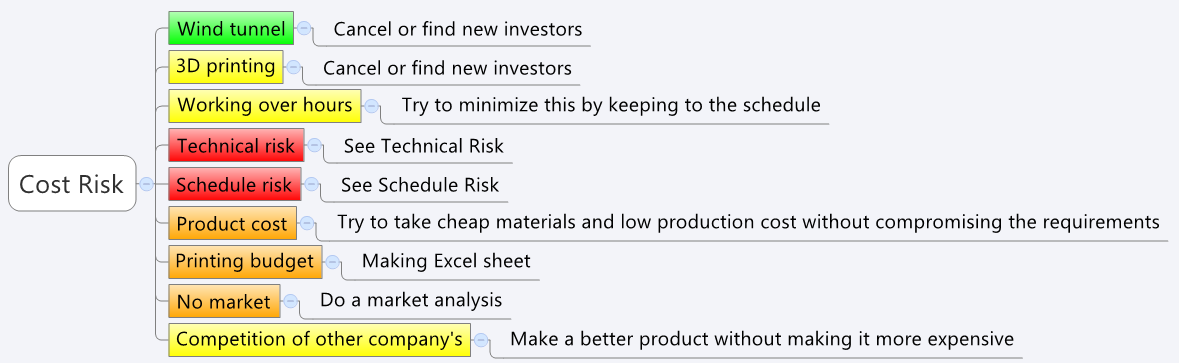
\includegraphics[scale=0.6]{Figures/riskmindcost.png}
\caption{The Contingency plan for the cost risk }
\end{figure}

The organizational risk sub group assesses the risks related to the organization of the workload. The most important things that can be learned from this sub group are that it is important to communicate, work on schedule and divide the work load as best as possible. 

\begin{figure}[H]
\label{fig:riskorgan}
\centering
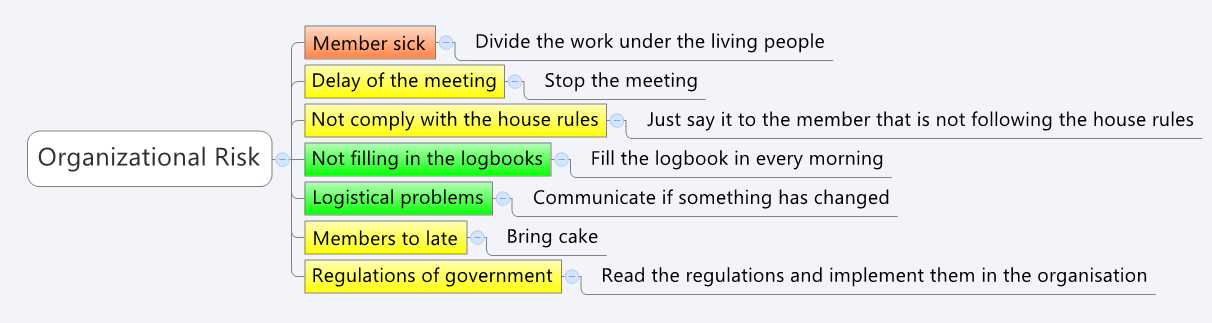
\includegraphics[scale=0.6]{Figures/riskmindorgan.png}
\caption{The technical risk map }
\end{figure}

The technical risk sub group assesses the risks related to technical issues. This is the largest group and the most important sub group. From this subgroup a Risk Map is made which is shown in section…. Special attention needs to be paid to this group since most of the solutions can be time consuming. 


\begin{figure}[H]
\label{fig:risktech}
\centering
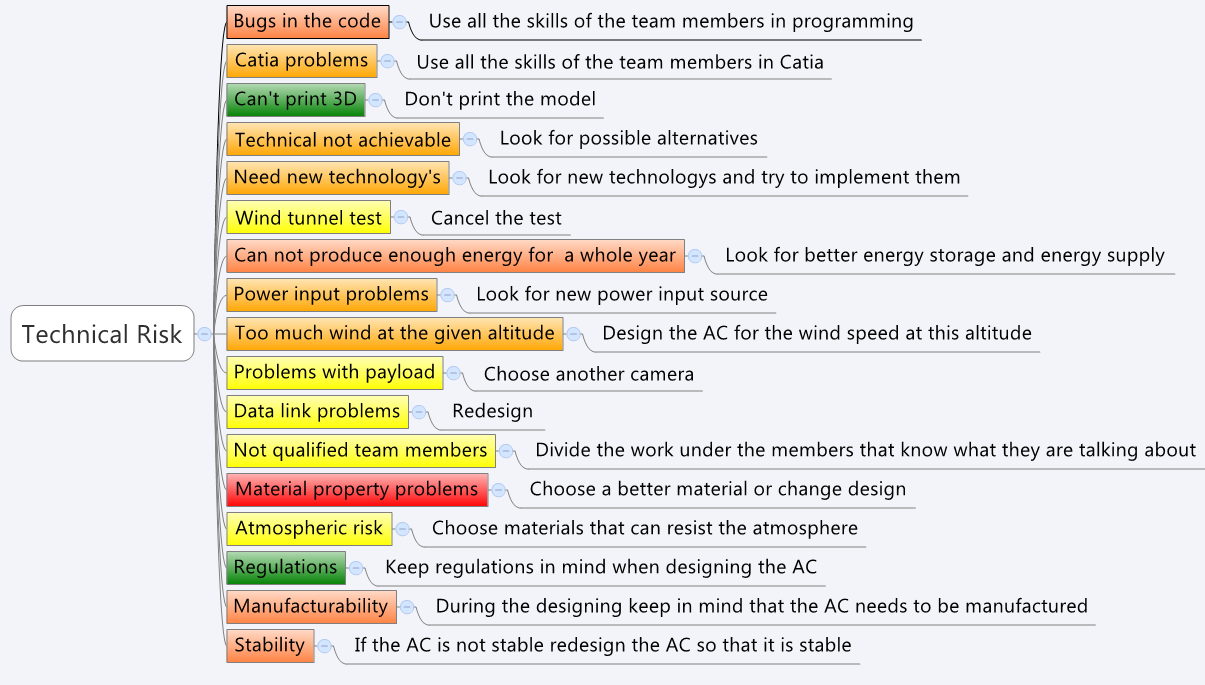
\includegraphics[scale=0.6]{Figures/riskmindtech.png}
\caption{The technical risk map }
\end{figure}

The schedule risk sub group assesses the risks related to the scheduling. It is clear from this sub group that it is important to keep on schedule and to keep planning up to date.  


\begin{figure}[H]
\label{fig:riskschedule}
\centering
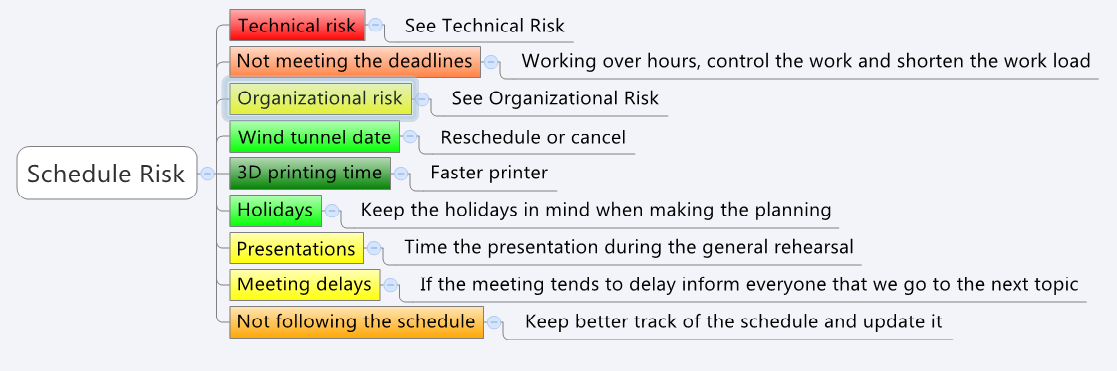
\includegraphics[scale=0.6]{Figures/riskmindschedule.png}
\caption{The technical risk map }
\end{figure}
\end{document}